\section{VL 09: Kontext Gesellschaft}
Informatik und Gesellschaft sind verzahnt!

\subsection{Definition: Gesellschaft}
Zwei Theorien:
\begin{itemize}
	\item Emile Durkheim:
	Die Gesellschaft beeinflusst und prägt das Individuum, ist eine "Realität eigener Art (= sui generis)", entstanden durch einen evolutionären Prozess und mehr als die Summe der Individuen.
	\item Max Weber:
	Gesellschaft ensteht durch individuelle Handlungen.
\end{itemize}
Die Emile Durkheim und Max Weber Definitionen setzen sich zusammen zu der Folgenden:

\emph{,,Gesellschaft = durch veränderliche, unterschiedliche Merkmale (Strukturen)
zusammengefasste und abgegrenzte Anzahl von Personen, die als soziale
Akteure miteinander verknüpft leben und direkt oder indirekt interagieren
(Handlungen) (Wikipedia 2012, mit Ergänzungen (in den Folien in rot))''}


\begin{center}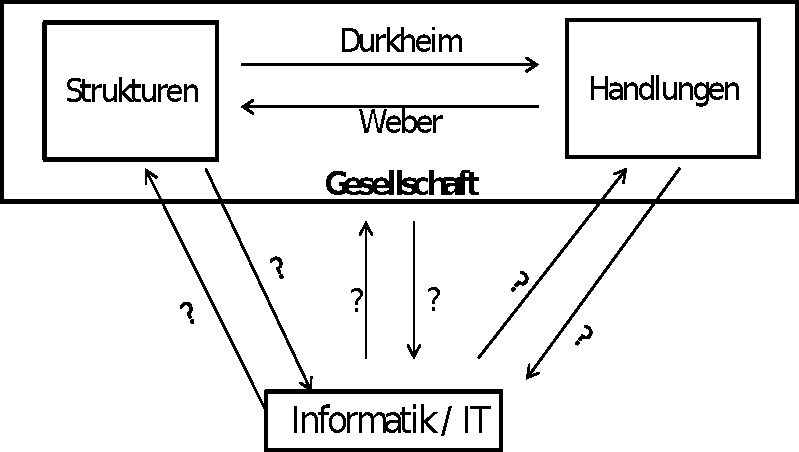
\includegraphics[width=0.7\textwidth]{9-1}\end{center}

\subsection{Welchen Einfluss hat IT also auf Gesellschaft, Strukturen und Handlungen?}

\begin{itemize}
\item Handlungen: 
	\begin{itemize}
		\item Wie bei Individuen bereits geklährt.
	\end{itemize}
\item Informatik beeinflusst Strukturen:
	\begin{itemize}
		\item Grundrecht informationelle Selbstbestimmung (Datenschutz):
			\begin{itemize}
				\item Grundrecht ging aus Volkszählung hervor, 1983 entschied Bundesverfassungsgericht, das es dieses Grundrecht durchs Grundgesetz (freie Entfaltung) impliziert wird.
				$ \rightarrow $ Datenschutz in Deutschland wird gefestigt 
				\item Datenvermeidung %& Sparsamkeit. (bisweilen in der Praxis nicht umgesetzt)
			\end{itemize}
		\item Bild der Informatik
			\begin{itemize}
				\item Typisches Klischee (Nerd)
				\item zugleich sehr gesuchte Berufsgruppe.
			\end{itemize}
	\end{itemize}

\item Strukturen beeinflussen die Informatik:
	\begin{itemize}
		\item Gesetze
		\item Werte, Kultur, Leitbilder 
		\item Arbeitsmarkt
	\end{itemize}
\item Informatik beeinflusst Strukturen:
		\begin{itemize}
		\item Web 2.0:
			\begin{itemize}
			\item Verändert Freizeitverhalten
			\item Arab Spring etc.
			\item Freiheit von Informationen etc.
			\item Internetsucht
			\end{itemize}
		\end{itemize}
\end{itemize}

Insgesamt beeinflusst Informatik Gesellschaftliche Strukturen durch neue Technologien und Innovationen sowie durch optimierte Prozesse (z.B. Technochange)

Da Handlungen und Strukturen durch IT beeinflusst werden, verändert sich entsprechend auch die gesamte Gesellschaft.